Utilizzando  GWT-RPC  tutte  le  chiamate  effettuate  dalla  pagina  HTML  al  server 
sono  asincrone.
Questo  significa  che  le  chiamate  non  bloccano  il  client  mentre attende   una 
risposta   dal   server,   ma   viene  eseguito   il   codice   immediatamente 
successivo.
\begin{figure}[!htb]
\centering%
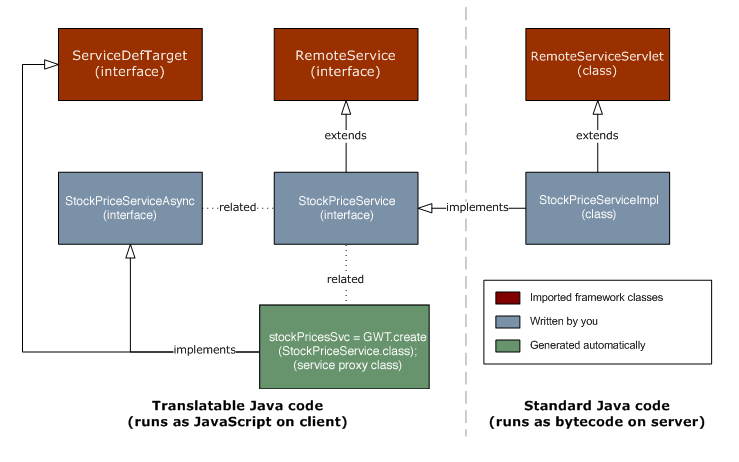
\includegraphics[scale=0.5]{AnatomyRPC.png}%
\caption{GWT-RPC }\label{fig:GWT-RPC}%
\end{figure}
I   vantaggi   di   effettuare   chiamate   asincrone   rispetto   alle   chiamate 
sincrone, si riscontrano in una migliore esperienza per gli utenti finali:
\begin{enumerate}
\item Interfaccia utente più reattiva, infat
ti, a causa del fatto che nei browserWeb il 
motore JavaScript è generalmente di tipo single-thread, una chiamata sincrona al 
server genera un "blocco" fino alla conclusione della stessa, rovinando così 
l’esperienza dell’utente finale.
\item Risulta possibile eseguire altri lavori in attesa della risposta da parte del server; 
per esempio, è possibile costruire l’interfaccia utente e contemporaneamente 
recuperare i dati dal server per popolarla, riducendo così il tempo complessivo 
necessario all’utente per visualizzare i dati sulla pagina.
\item E’ possibile effettuare chiamate multiple al server nello stesso tempo.
\end{enumerate}